\documentclass[11pt]{scrartcl}       % KOMA-Skript für Artikel
	
%% Präambel
\setlength{\parindent}{0pt}
\usepackage[english, ngerman]{babel} % deutsche typogr. Regeln + Trenntabelle
\usepackage[T1]{fontenc}             % interner TeX-Font-Codierung
      % Font Latin Modern
\usepackage[utf8]{inputenc}          % Font-Codierung der Eingabedatei
\usepackage[babel]{csquotes}         % Anführungszeichen
\usepackage{graphicx}                % Graphiken
\usepackage{booktabs}                % Tabellen schöner
\usepackage{listingsutf8}            % Listings mit Einstellungen
\usepackage{listings}
\usepackage{color}
\usepackage{subfig}

\definecolor{dkgreen}{rgb}{0,0.6,0}
\definecolor{gray}{rgb}{0.5,0.5,0.5}
\definecolor{mauve}{rgb}{0.58,0,0.82}

\lstset{frame=tb,
  language=Java,
  aboveskip=5mm,
  belowskip=5mm,
  showstringspaces=false,
  columns=flexible,
  basicstyle={\small\ttfamily},
  numbers=none,
  numberstyle=\tiny\color{gray},
  keywordstyle=\color{blue},
  commentstyle=\color{dkgreen},
  stringstyle=\color{mauve},
  breaklines=true,
  breakatwhitespace=true,
  tabsize=5
}
\lstset{basicstyle=\small\ttfamily,
	tabsize=2,
	basewidth={0.5em,0.45em},
	extendedchars=true}
\usepackage{amsmath}	               % Mathematik
\usepackage[pdftex]{hyperref}       
\hypersetup{
	bookmarksopen=true,
	bookmarksopenlevel=3,
	colorlinks,
	citecolor=blue,
	linkcolor=blue,
}
\usepackage{scrhack}								 % unterdrückt Fehlermeldung von listings

%% Nummerierungstiefen
\setcounter{tocdepth}{3}             % 3 Stufen im Inhaltsverzeichnis
\setcounter{secnumdepth}{3} 		     % 3 Stufen in Abschnittnummerierung

% ----------------------------------------------------------------------------
\begin{document}
\titlehead{

\includegraphics[width=0.9\textwidth]{img/mni-logo}
}
\subject{Course \glqq Secure Software Engineering\grqq}
\title{Setting up IPFire Server}
\author{Autor: }
\date{Sommersemester 2019}
\publishers{Betreut von\\ Prof. Dr. Muster}
\maketitle
\newpage
\tableofcontents
\newpage

\section{Einführung und Aufbau}
Im echten Leben wird man normalerweise mit verteilten Systemen konfrontiert. 
\textbf{Transaktion} und \textbf{verteilten Transaktion} unterschieden. 
\\\\

% Schwierigkeiten in den verteilten Transaktionen 
% werden im Kapitel~\ref{sec:kapitel2} beschrieben. Im Kapitel~\ref{sec:kapitel3} wird ein möglicher Lösungsansatz für die Schwierigkeiten aus dem Kapitel~\ref{sec:kapitel2} vorgeschlagen und die Grundlagen des 2PCs erklärt. Mögliche Alternativen zu 2PC werden im Kapitel~\ref{sec:kapitel4} genannt.

\section{Problemstellung}\label{sec:kapitel2}
\subsection{ACID Eigenschaften}
\begin{itemize}
	\item \textbf{A}tomicity - alle Schritte der Transaktion werden als unteilbare Einheit ausgeführt.
	\item \textbf{C}onsistency - Datenbank ist nach der Transaktion immer noch im konsistenten Zustand.
	\item \textbf{I}solation - Transaktion ist von den anderen Transaktionen isoliert.
	\item \textbf{D}urability - Ergebnisse der Transaktion werden dauerhaft gesichert. 
\end{itemize}

\subsection{Beispiel aus dem Leben}

Durch ein einfaches Beispiel kann die Problematik der 
verteilten Transaktionen besser dargestellt werden: 

\begin{itemize}
	\item
	\textbf{T\textsubscript{1}} Von dem Konto 1 \$100 umbuchen.
	\item
	\textbf{T\textsubscript{2}} Von dem Konto 2 \$100 umbuchen.
	\item
	\textbf{T\textsubscript{3}} Von dem Konto 3 \$100 umbuchen. 
	\item 
	\textbf{T\textsubscript{4}} Auf das vierte Konto 3 * \$100 gutschreiben. 
\end{itemize}

\begin{lstlisting}[language=SQL, caption=Transaktion als SQL dargestellt]
	begin transaction --T
		update Konto @StandortA set Saldo = Saldo - 100 where KontoNr = 1; --T1
		update Konto @StandortB set Saldo = Saldo - 100 where KontoNr = 2; --T2
		update Konto @StandortC set Saldo = Saldo - 100 where KontoNr = 3; --T3
		update Konto @StandortD set Saldo = Saldo + 300 where KontoNr = 4; --T4
	commit;
\end{lstlisting}

\begin{enumerate}
	\item Auf einem von den 3 Konten ist nicht genug Geld, sodass eine von \textbf{T\textsubscript{1}}-\textbf{T\textsubscript{3}} abgebrochen wird. Nachdem die  Transaktion T\textsubscript{4} ausgeführt wird, geht das Gesamtsystem in den inkonsistenten Zustand über (3 x \$100 gutgeschrieben, obwohl eine der \textbf{T\textsubscript{1}}-\textbf{T\textsubscript{3}} fehlgeschlagen). 
	\item Einer von 3 Servern stürzt während der Transaktion ab und eine der \textbf{T\textsubscript{1}}-\textbf{T\textsubscript{3}} schlägt fehl, was das Gesamtsystem zum inkonsistenten Zustand führt.
	\item Der vierte Server stürzt vor der Transaktion T\textsubscript{4} ab, was wieder das Gesamtsystem zum inkonsistenten Zustand führt. \cite{database_systems}
\end{enumerate}

\section{2-Phasen-Commit Protokoll}\label{sec:kapitel3}
\subsection{2PC Grundlagen}
Im 2-Phasen-Commit-Protokoll wird zwischen 
dem \textbf{Koordinator}, der die verteilte Transaktion steuert, und den \textbf{Teilnehmern}, an denen die Komponententransaktionen durchgeführt werden, unterschieden.

\subsubsection{Wahlphase}
Die endlichen Automaten [\ref{fig:participant2pc-label}] repräsentieren
den Ablauf des 2PC Protokolls. Dies funktioniert folgendermaßen:
\begin{itemize}
	\item Teilnehmer ist z.B im INIT Zustand.
	\item Teilnehmer bekommt von Koordinator eine vote-request Nachricht.
	\item Teilnehmer hat zwei Möglichkeiten: vote-commit zu versenden und \
	in den READY Zustand oder mit vote-abort in den ABORT Zustand zu wechseln.
\end{itemize}

\begin{enumerate}
	\item Koordinator verschickt vote-request \
	Nachricht an alle Teilnehmer. 
	\item Nachdem die Teilnehmer vote-request bekommen haben, 
	antworten sie entweder mit vote-commit 
	(Teiltransaktion wurde erfolgreich ausgeführt) 
	oder \mbox{vote-aborted} (Teiltransaktion wurde
	 rückgängig gemacht).
\end{enumerate}
\subsubsection{Durchführungsphase}
In der Durchführungsphase geht es darum, die verteilte 

\subsection{Blockierung des Protolkolls}
\label{sec:blocking}

\begin{figure}[!tbp]
	\centering
	\subfloat[DEA des Teilnehmers]{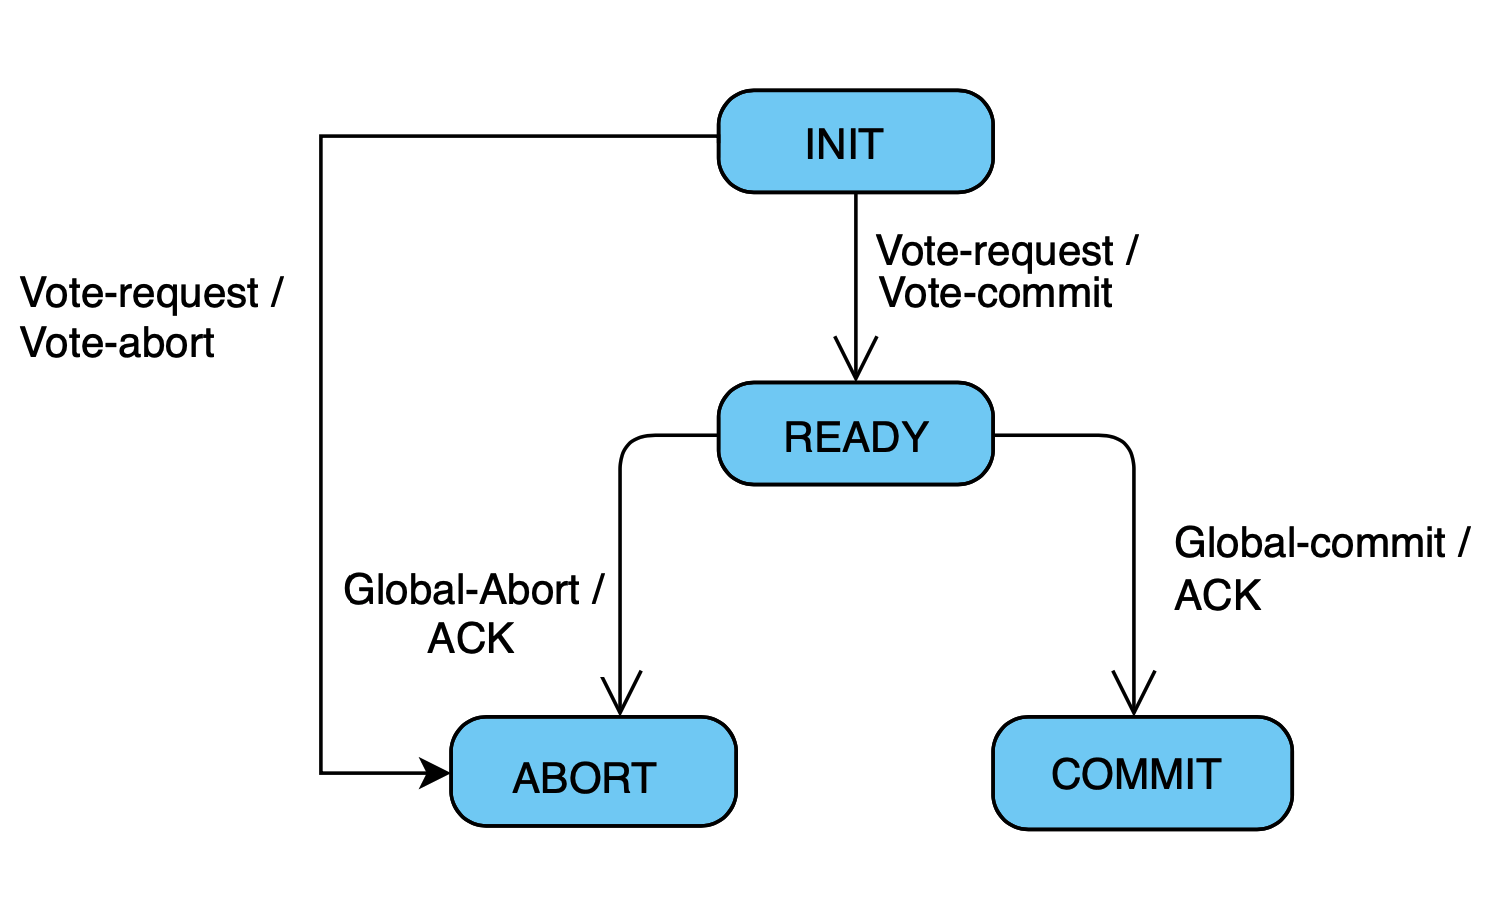
\includegraphics[width=0.5\textwidth]{img/participant2pc.png}}
	\hfill
	\subfloat[DEA des Koordinators]{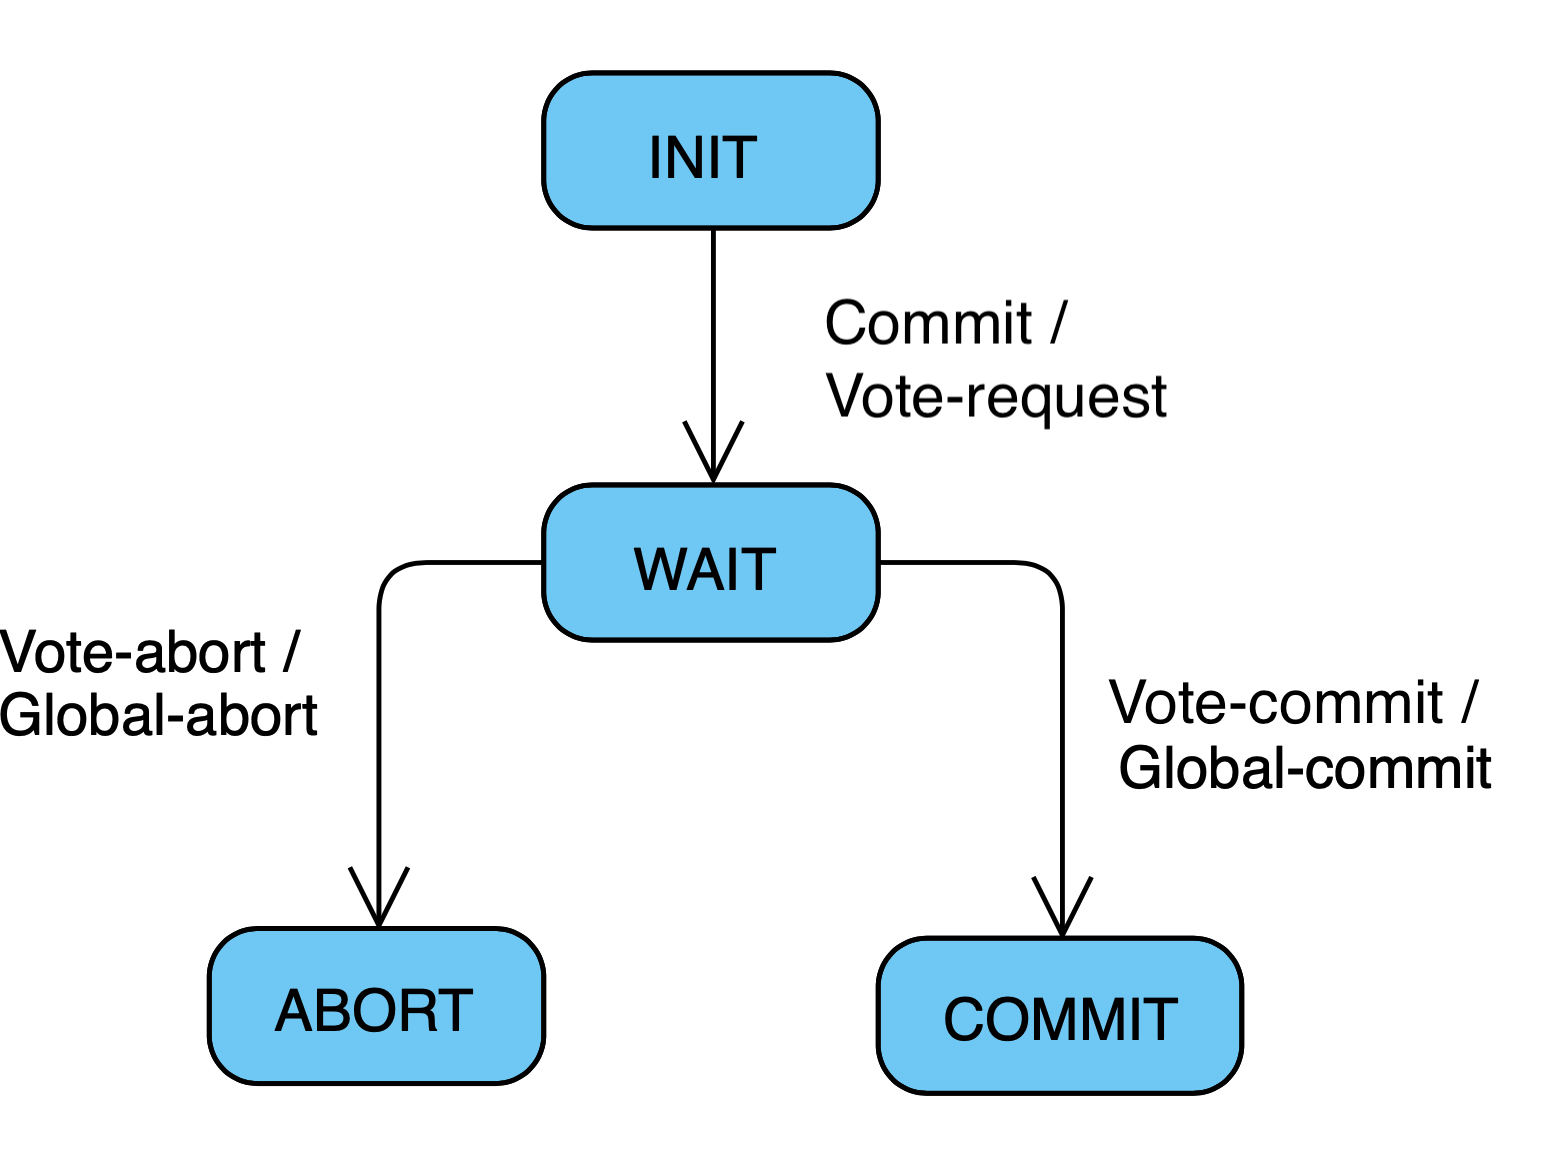
\includegraphics[width=0.4\textwidth]{img/coordinator2pc.png}}
	\caption{Deterministische Endliche Automaten des Koordinators und Teilnehmers im 2PC}
	\label{fig:participant2pc-label}
\end{figure}

\section{3PC als Alternative zu 2PC}\label{sec:kapitel4}
Um Blockierungen aus dem Kapitel~\ref{sec:blocking}
gleichzeitig zum \textbf{ABORT} oder \textbf{COMMIT} 
Zustand übergehen kann [\ref{fig:participant3pc-label}].

\begin{figure}[!tbp]
	\centering
	\subfloat[DEA des Teilnehmers]{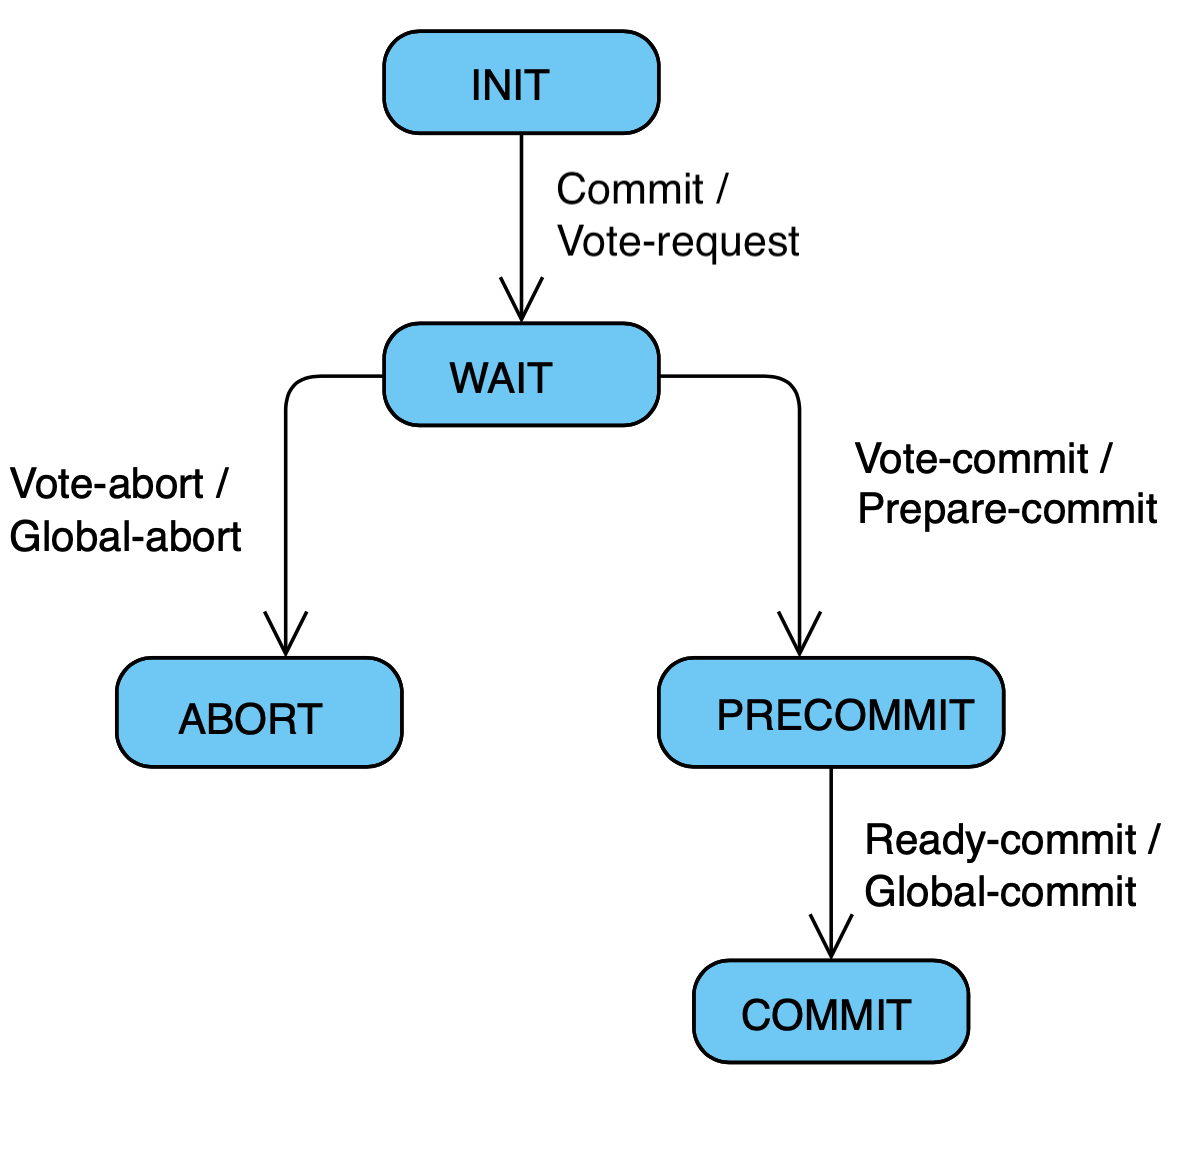
\includegraphics[width=0.4\textwidth]{img/3pc_coordinator.png}}
	\hfill
	\subfloat[DEA des Koordinators]{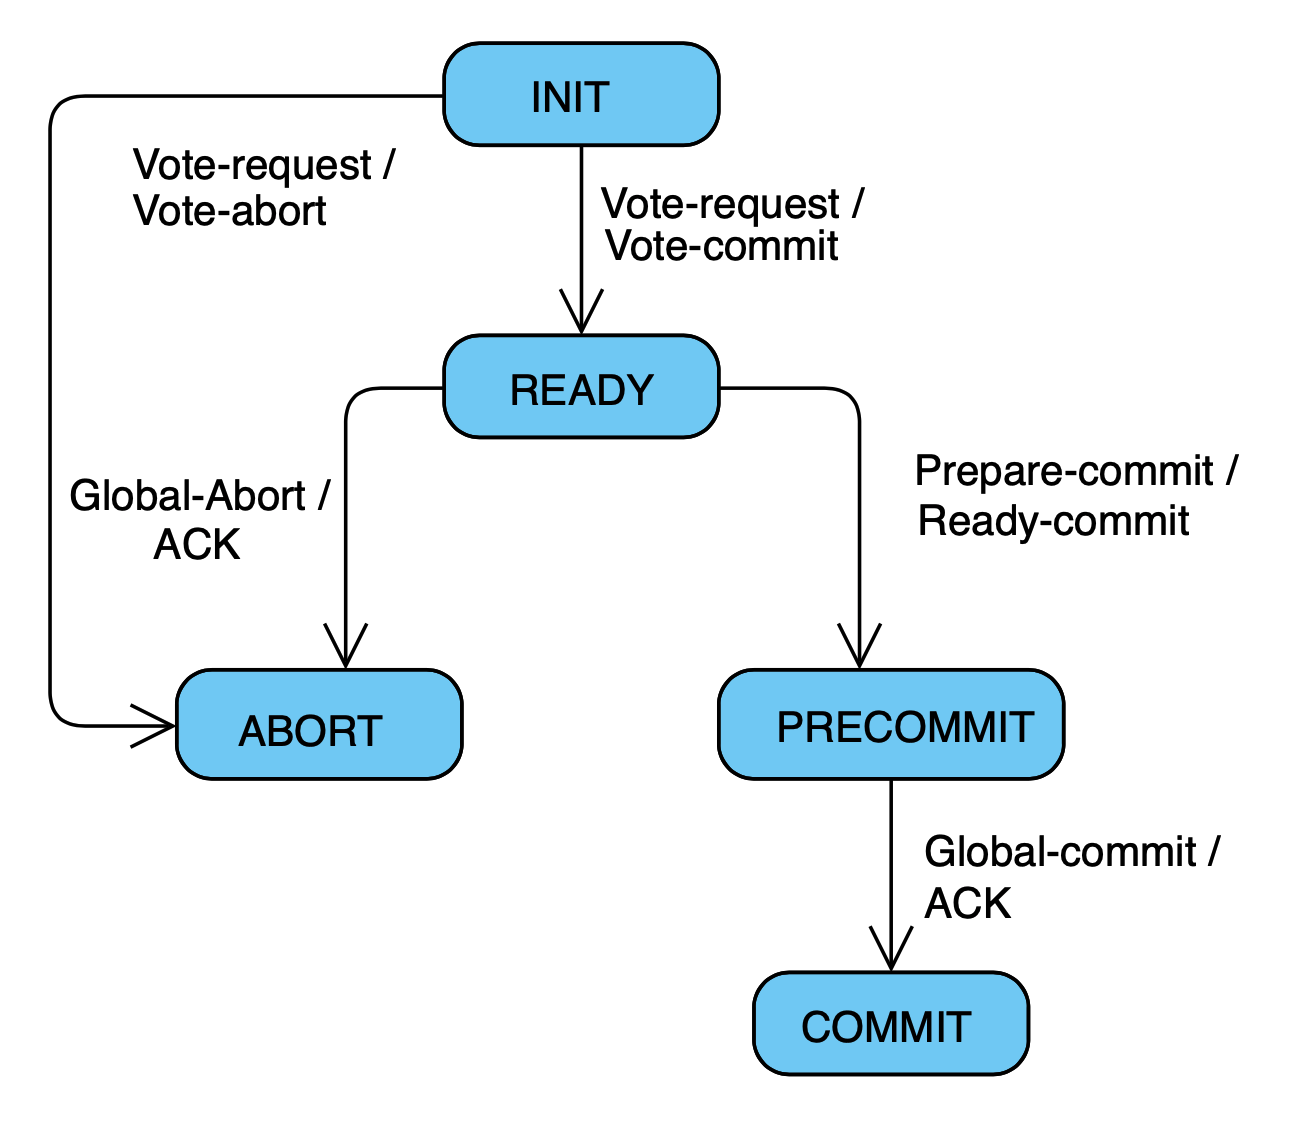
\includegraphics[width=0.4\textwidth]{img/3pc_participant.png}}
	\caption{Deterministische Endliche Automaten des Koordinators und Teilnehmers im 3PC}
	\label{fig:participant3pc-label}
\end{figure}

\section{Fazit}\label{sec:kapitel5}

\newpage
\section{Literaturverzeichnis}
\begin{thebibliography}{99}                    % max. 99 Einträge möglich
	
\bibitem{tannenbaum_distsystems}
	Andrew S. Tanenbaum, Maarten Van Steen 
	\emph{Distributed Systems Principles und Paradigms second edition},
	Pearson Prentice Hall ISBN 0-13-239227-5
	
\bibitem{database_systems}
Hector Garcia-Molina Jeffrey D. Ullman Jennifer Widom	
	\emph{Database Systems The Complete Book
	Second Edition},
	Pearson Prentice Hall ISBN 0-13-239227-5
\end{thebibliography}

\end{document}
% ----------------------------------------------------------------------------

